\documentclass{libs/ccnu_format}
\usepackage{kerkis}
\usepackage{kmath}
\usepackage{ctex,hyperref}
\usepackage{calligra}
\usepackage{amsmath}
\usepackage{makecell}
\usepackage{multirow}
\usepackage{amsfonts}
\usepackage{booktabs}
\usepackage{mathrsfs}
\usepackage{pifont}
\usepackage{amssymb}
\usepackage[T1]{fontenc}
\usepackage{tcolorbox}
\usepackage[T1]{fontenc}
\usepackage[utf8]{inputenc}
\usepackage[brazil]{babel}
\usepackage{graphicx}
\usepackage{color}
\usepackage{xcolor}
\usepackage{amsfonts, amssymb, amsmath}
\usepackage{multirow, array} 
\usepackage{algorithm2e}
\usepackage{listings} 
\usepackage{keyval}
\usepackage[document]{ragged2e}
\usepackage[backend=bibtex,sorting=none]{biblatex}
\usepackage{csquotes}
\usepackage{multicol}
\defbibheading{bibliography}[\bibname]{}
\addbibresource{references.bib}
\setbeamertemplate{bibliography item}{\insertbiblabel}

\title[\LaTeX{}与科研]{\huge\bfseries{为你的学术科研做更专业的 Presentation}}
\subtitle{\bfseries 华中师范大学}
\author{Banach Spaces}
\institute[CCNU]{
    % email for contact
    \normalsize{\email{yongxuel487@foxmail.com}}
    \newline
    \department{数学与统计学学院}
    \newline
    \ccnu
}
\date{January 28, 2021}


%%%%%%%%%%%%%%%%%%%%%%%%%%%%%%%%%%%%%%%%%%%%%%%%%%%%%%%%%%%%%%%%%%%%%%%%%%%%%%%%%%
%% Start Document of the Presentation                                           %%
%%%%%%%%%%%%%%%%%%%%%%%%%%%%%%%%%%%%%%%%%%%%%%%%%%%%%%%%%%%%%%%%%%%%%%%%%%%%%%%%%%
\begin{document}

% insert the code style
%%%%%%%%%%%%%%%%%%%%%%%%%%%%%%%%%%%%%%%%%%%%%%%%%%%%%%%%%%%%%%%%%%%%%%%%%%%%%%%%%%%
%% This file contains the style of the codes show in slides.                     %%
%% The package used is listings, but it possible to used others.                 %%
%%%%%%%%%%%%%%%%%%%%%%%%%%%%%%%%%%%%%%%%%%%%%%%%%%%%%%%%%%%%%%%%%%%%%%%%%%%%%%%%%%%

% color used in the code style
\definecolor{codegreen}{rgb}{0,0.6,0}
\definecolor{codegray}{rgb}{0.5,0.5,0.5}
\definecolor{codepurple}{rgb}{0.58,0,0.82}
\definecolor{codebackground}{rgb}{0.95,0.95,0.92}

% style of the code!
\lstdefinestyle{codestyle}{
    backgroundcolor=\color{codebackground},
    commentstyle=\color{codegreen},
    keywordstyle=\color{magenta},
    numberstyle=\tiny\color{codegray},
    morestring=[s][\bfseries\color{red}]{\[}{\]},
    morestring=[s][\bfseries\color{blue}]{\{}{\}},
    stringstyle=\color{codepurple},
    basicstyle=\ttfamily\footnotesize,
    frame=single,
    breakatwhitespace=false,
    breaklines=true,
    captionpos=b,
    keepspaces=true,
    numbers=left,
    numbersep=5pt,
    showspaces=false,
    showstringspaces=false,
    showtabs=false,
    tabsize=2,
    title=\lstname
}

\lstset{style=codestyle}


%% ---------------------------------------------------------------------------
% First frame (with tile, subtitle, ...)
\begin{frame}{}
    \maketitle
\end{frame}
\kaishu
%% ---------------------------------------------------------------------------
\begin{frame}{目\quad 录}
\begin{multicols}{2}
        \tableofcontents
\end{multicols}
\end{frame}

%% ---------------------------------------------------------------------------
% This presentation is separated by sections and subsections
\section{理论基础}
\begin{frame}{内容概要}
这部分我们先在这里介绍本部分内容的大致架构:
\begin{multicols}{2}

数学公式
    \begin{itemize}
        \item 行内公式
        \item 行间公式
    \end{itemize}

\vspace{0.2cm}

绘图与插图

    \begin{itemize}
        \item TikZ/PGFplots绘图
        \item 插入多张图
        \item Tikzpicture 环境与插图
    \end{itemize}

\vspace{0.2cm}
表格环境
    \begin{enumerate}
    \item 三线表格
    \item Diagbox
    \item tabu 表格
    \item 其他
    
    \vspace{0.2cm}
    代码摘录
    \begin{enumerate}
    \item Algoritmos 代码
    \item Python 代码
    \item C 语言代码
    \item Java 语言代码
    \item HTML 代码
\end{enumerate}

    \end{enumerate}
\end{multicols}
\end{frame}

%% ---------------------------------------------------------------------------
\subsection{支撑项目的基础理论}
\begin{frame}{基础理论}

    \begin{block}{定理 1(Tonelli 定理)}
       设  $f(x, y)$  是  $\mathbb{R}^{n}=\mathbb{R}^{p} \times \mathbb{R}^{q}$  上的非负的广义实值
L-可测 函数, 则
(A) 对几乎处处的  $x \in \mathbb{R}^{p}$, $f(x, y)$  作为  $y$  的函数 是  $\mathbb{R}^{q}$  上的非负的 L-可测函数;
(B) $记  F_{f}(x)=\int_{\mathbb{R}^{q}} f(x, y) \rm{d} y$,  则  $F_{f}$  是  $\mathbb{R}^{p}$  上的
非负的 L-可测 函数;
(C)  $\int_{\mathbb{R}^{n}} f(x, y) \rm{d} x \rm{d} y=\int_{\mathbb{R}^{p}}\left(\int_{\mathbb{R}^{q}} f(x, y) \rm{d} y\right) \rm{d} x$.
    \end{block}

    \begin{exampleblock}{引理~I}
(1) 若  $f \in \mathscr{F}$, $\alpha \geq 0$,  则  $\alpha f \in \mathscr{F}$.

(2) 若  $f, g \in \mathscr{F}$,  则  $f+g \in \mathscr{F}$.

(3) 若  $f, g \in \mathscr{F}$, $f \geq g$,  且  $g $ 可积, 则  $f-g \in \mathscr{F}$.

(4) 若  $f_{k} \in \mathscr{F}$, $f_{k} \leq f_{k+1}$  (其中  $k=1,2, \cdots$) ,
且  $\lim _{k \rightarrow \infty} f_{k}=f$,  则  $f \in \mathscr{F}$.
    \end{exampleblock}

\end{frame}

%% ---------------------------------------------------------------------------
\subsection{应用与实践}
\begin{frame}{}

 \begin{tcolorbox}[title=\textbf{例 3 (Gaussian 积分)},colback=violet!60!blue!10,colframe=Deepblue!55!wine!100!]
 $\int_{-\infty}^{+\infty} \mathrm{e}^{-x^{2}} \rm{d} x=\sqrt{\pi}$
 \end{tcolorbox}

 \begin{tcolorbox}
   [colback=gray!10,colframe=Orange!40!blue!60!black,title=\textbf{证明}]
   设  $f(x, y)=y \mathrm{e}^{-\left(1+x^{2}\right) y^{2}}$ .  则  $f$  在  $\mathbb{R}^{2}$  上非负. $\int_{0}^{+\infty}\left(\int_{0}^{+\infty} f(x, y) \mathrm{d} y\right) \mathrm{d} x=\frac{\pi}{4}$.

   \end{tcolorbox}

 \begin{tcolorbox}
     [title = \textbf{续证}, colback=pink!20, colframe=green!40!yellow!50!violet]
     由 Tonelli 定理知  $\int_{(0,+\infty)^{2}} f(x, y) \rm{d} x \rm{d} y=\frac{\pi}{4}$,  故可
交换积分次序, 从而有
$\left(\int_{0}^{+\infty} e^{-x^{2}} d x\right)^{2}=\frac{\pi}{4}$.
     \end{tcolorbox}

\end{frame}

%% ---------------------------------------------------------------------------
\section{TikZ 绘图与 figure环境}
\subsection{Figure环境}
\begin{frame}{Figure 插图与TikZ 绘图}

\begin{figure}
        \centering
        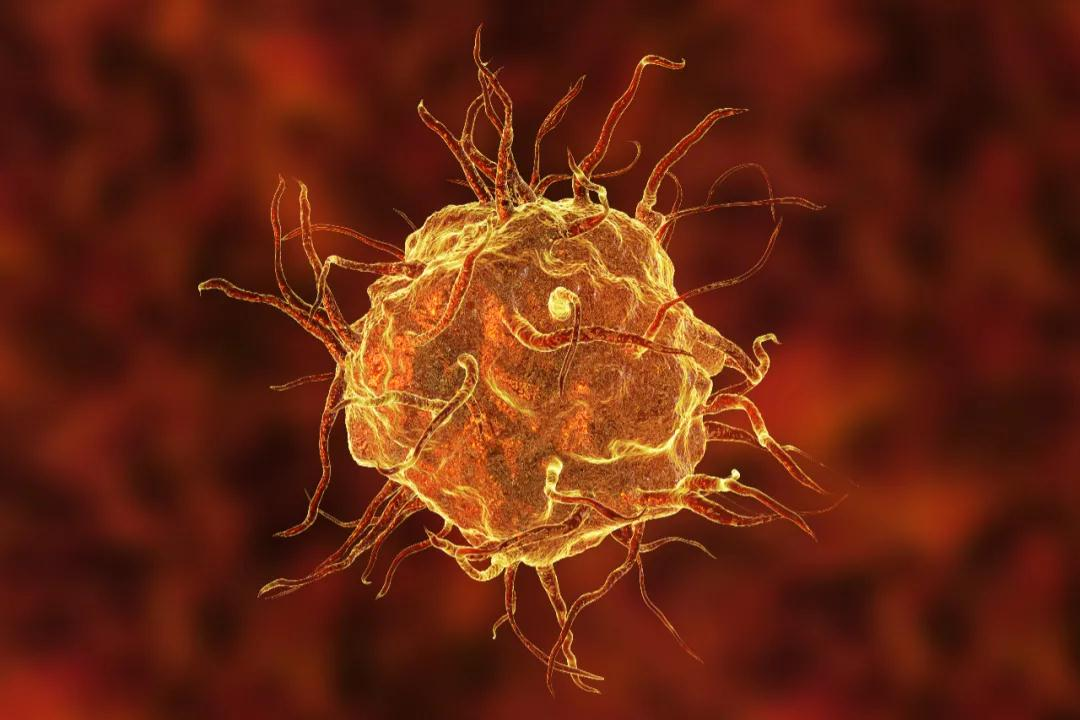
\includegraphics[scale=0.3]{libs/cell.jpg}

        \caption{Phagocyte}\source{KATERYNAKON/SCIENCE PHOTO LIBRARY/GETTY}

        \label{fig:ufc_emblem}
    \end{figure}


\end{frame}

%% ---------------------------------------------------------------------------
\subsection{TikZ 绘图}
\begin{frame}{TikZ 绘图}

\begin{figure}
        \centering
        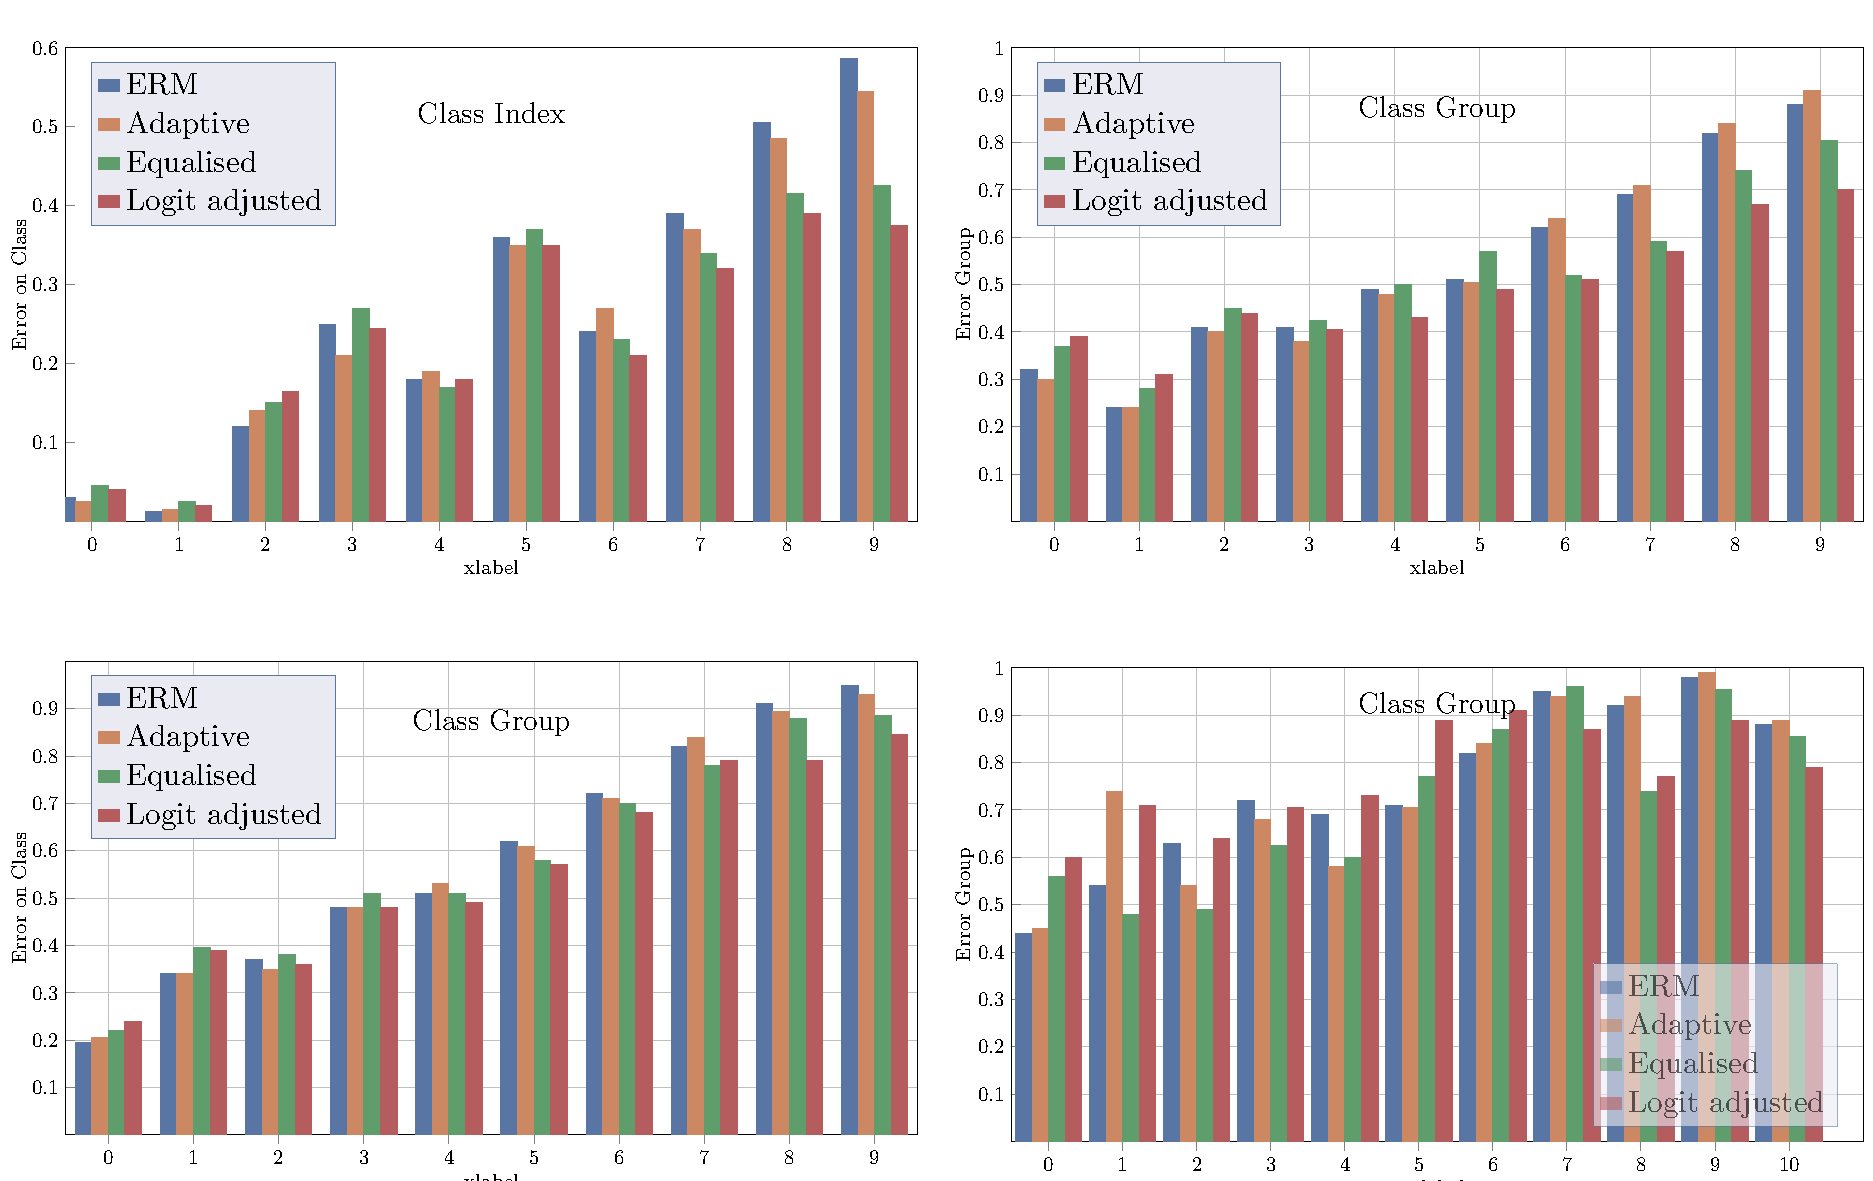
\includegraphics[scale=0.3]{libs/Data1.pdf}

        \caption{Comparison of different data.}

        \source{KATERYNAKON/SCIENCE PHOTO LIBRARY/GETTY}
        \label{fig:ufc_emblem}
    \end{figure}

sxusu
susu

\end{frame}



%% ---------------------------------------------------------------------------
% This frame show an example to insert figures

\begin{frame}{TikZ 绘图}
    \begin{figure}
        \centering
        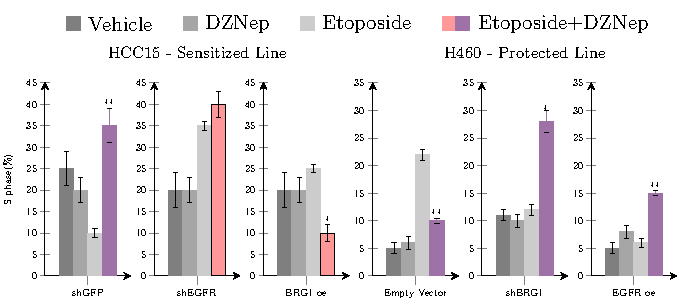
\includegraphics[scale=1]{libs/Data.pdf}
        \caption{Comparison of different data.}
        %\source{图片来源:http://maths.ccnu.edu.cn/}
        \label{fig:ufc_emblem}
    \end{figure}


\end{frame}

%% ---------------------------------------------------------------------------
\section{表格数据}
\begin{frame}{数据与tabular环境}
\begin{table}[H]
    \tiny
  \centering
  %\setlength{\tabcolsep}{-3pt}
  \resizebox{!}{3.0cm}{\begin{tabular}{@{\extracolsep{\fill}}*{3}{l}}
\toprule
    Category of your contents & Different types of each  Category & other type of  your data \\
    \midrule
    &\multicolumn{2}{c}{\hrulefill~~ tha$\theta^{-1}$kg ~~\hrulefill}\\
\multirow{12}{*}{Type of date (numbers)}
    & 0.0056 $\pm$ 0.0097, 0.0021 $\pm$ 4.0056 & 3.5 $\times$ 10$^{5}$ ; 5.43 (9.30\%) \\
    & 0.0056 $\pm$ 0.0097, 0.0021 $\pm$ 4.0056 & 3.5 $\times$ 10$^{5}$ ; 5.43 (9.30\%) \\
    & 0.0056 $\pm$ 0.0097, 0.0021 $\pm$ 4.0056 & 3.5 $\times$ 10$^{5}$ ; 5.43 (9.30\%) \\
    & 0.0056 $\pm$ 0.0097, 0.0021 $\pm$ 4.0056 & 3.5 $\times$ 10$^{5}$ ; 5.43 (9.30\%) \\
    & 0.0056 $\pm$ 0.0097, 0.0021 $\pm$ 4.0056 & 3.5 $\times$ 10$^{5}$ ; 5.43 (9.30\%) \\
    & 0.0056 $\pm$ 0.0097, 0.0021 $\pm$ 4.0056 & 3.5 $\times$ 10$^{5}$ ; 5.43 (9.30\%) \\
    & 0.0056 $\pm$ 0.0097, 0.0021 $\pm$ 4.0056 & 3.5 $\times$ 10$^{5}$ ; 5.43 (9.30\%) \\
    & 0.0056 $\pm$ 0.0097, 0.0021 $\pm$ 4.0056 & 3.5 $\times$ 10$^{5}$ ; 5.43 (9.30\%) \\
    & 0.0056 $\pm$ 0.0097, 0.0021 $\pm$ 4.0056 & 3.5 $\times$ 10$^{5}$ ; 5.43 (9.30\%) \\
    & 0.0056 $\pm$ 0.0097, 0.0021 $\pm$ 4.0056 & 3.5 $\times$ 10$^{5}$ ; 5.43 (9.30\%) \\
    & 0.0056 $\pm$ 0.0097, 0.0021 $\pm$ 4.0056 & 3.5 $\times$ 10$^{5}$ ; 5.43 (9.30\%) \\
    & 0.0056 $\pm$ 0.0097, 0.0021 $\pm$ 4.0056 & 3.5 $\times$ 10$^{5}$ ; 5.43 (9.30\%) \\
    \hline
\multirow{3}{*}{Mathematical formulas}
   & $\frac{\mu^2}{\pi-2\theta}\times \sqrt[3]{\|\nu_{i}-\hat{\phi\|}}+\lim\limits_{s\to\infty}\int_{0}^{+\infty}f(x)e^{xsi}{\rm d}x$ & $f(x)\in C^{1}[0,+\infty]$, $\|f(x^{n})\|_{2}\leqslant \lambda$ \\
   &$\frac{\mu^2}{\pi-2\theta}\times \sqrt[3]{\|\nu_{i}-\hat{\phi\|}}+\lim\limits_{s\to\infty}\int_{0}^{+\infty}f(x)e^{xsi}{\rm d}x$ & $f(x)\in C^{1}[0,+\infty]$, $\|f(x^{n})\|_{2}\leqslant \lambda$ \\
   & $\frac{\mu^2}{\pi-2\theta}\times \sqrt[3]{\|\nu_{i}-\hat{\phi\|}}+\lim\limits_{s\to\infty}\int_{0}^{+\infty}f(x)e^{xsi}{\rm d}x$ & $f(x)\in C^{1}[0,+\infty]$, $\|f(x^{n})\|_{2}\leqslant \lambda$ \\
   \hline
\multirow{7}{*}{Language description}
    & This is the element described in your language & Mathematical language description \\
    & This is the element described in your language & Mathematical language description\\
    & This is the element described in your language & Mathematical language description \\
    & This is the element described in your language & Mathematical language description \\
    & This is the element described in your language & Mathematical language description \\
    & This is the element described in your language & Mathematical language description\\
    & This is the element described in your language & Mathematical language description\\
    \hline
\multirow{8}{*}{Projection data}
    & 3.5 $\times$ 10$^{5}$ This is the element described in your language&  0.0056 $\pm$ 0.0097, 0.0021 $\pm$ 4.0056 \\
    & 3.5 $\times$ 10$^{5}$ This is the element described in your language&  0.0056 $\pm$ 0.0097, 0.0021 $\pm$ 4.0056 \\
    & 3.5 $\times$ 10$^{5}$ This is the element described in your language&  0.0056 $\pm$ 0.0097, 0.0021 $\pm$ 4.0056 \\
    & 3.5 $\times$ 10$^{5}$ This is the element described in your language&  0.0056 $\pm$ 0.0097, 0.0021 $\pm$ 4.0056 \\
    & 3.5 $\times$ 10$^{5}$ This is the element described in your language&  0.0056 $\pm$ 0.0097, 0.0021 $\pm$ 4.0056 \\
    & 3.5 $\times$ 10$^{5}$ This is the element described in your language&  0.0056 $\pm$ 0.0097, 0.0021 $\pm$ 4.0056\\
    & 3.5 $\times$ 10$^{5}$ This is the element described in your language&  0.0056 $\pm$ 0.0097, 0.0021 $\pm$ 4.0056 \\
    & 3.5 $\times$ 10$^{5}$ This is the element described in your language&  0.0056 $\pm$ 0.0097, 0.0021 $\pm$ 4.0056 \\
    & 3.5 $\times$ 10$^{5}$ This is the element described in your language&  0.0056 $\pm$ 0.0097, 0.0021 $\pm$ 4.0056 \\
\bottomrule
  \end{tabular}
  }
  \caption{Contents of different types of tables.}
\end{table}

\end{frame}

% ----------------------------------------------------------------------------
\begin{frame}{}
\noindent
    \begin{minipage}{0.4\linewidth}
    \begin{figure}[H]
       \centering
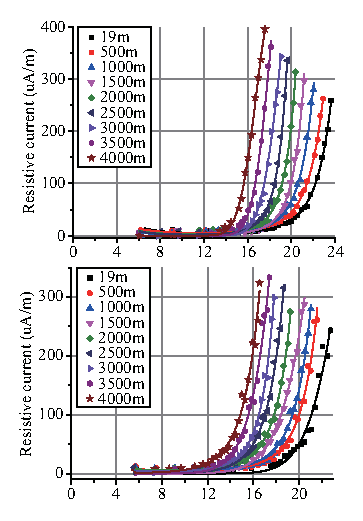
\includegraphics[scale=0.8]{libs/Graphic.eps}
\caption{\footnotesize WMA method overview.}
\end{figure}
    \end{minipage}\quad
    \begin{minipage}{0.55\linewidth}
\begin{table}[H]
    \tiny
  \centering
  %\setlength{\tabcolsep}{-3pt}
  \resizebox{!}{3.5cm}{\begin{tabular}{lll}
\toprule
    Tract category (tract\#) & Tract name &\\
\midrule
    0.0056 $\pm$ 0.0097, 0.0021 $\pm$ 4.0056 & 0.0056 $\pm$ 0.0097, 0.0021 $\pm$ 4.0056 &  0.0056 $\pm$ 0.0097, 0.0021 $\pm$ 4.0056\\
    0.0056 $\pm$ 0.0097, 0.0021 $\pm$ 4.0056 & 0.0056 $\pm$ 0.0097, 0.0021 $\pm$ 4.0056 &  0.0056 $\pm$ 0.0097, 0.0021 $\pm$ 4.0056\\
    0.0056 $\pm$ 0.0097, 0.0021 $\pm$ 4.0056 & 0.0056 $\pm$ 0.0097, 0.0021 $\pm$ 4.0056 &  0.0056 $\pm$ 0.0097, 0.0021 $\pm$ 4.0056\\
    0.0056 $\pm$ 0.0097, 0.0021 $\pm$ 4.0056& 0.0056 $\pm$ 0.0097, 0.0021 $\pm$ 4.0056 &  0.0056 $\pm$ 0.0097, 0.0021 $\pm$ 4.0056\\
    0.0056 $\pm$ 0.0097, 0.0021 $\pm$ 4.0056& 0.0056 $\pm$ 0.0097, 0.0021 $\pm$ 4.0056 &  0.0056 $\pm$ 0.0097, 0.0021 $\pm$ 4.0056\\
    0.0056 $\pm$ 0.0097, 0.0021 $\pm$ 4.0056& 0.0056 $\pm$ 0.0097, 0.0021 $\pm$ 4.0056 &  0.0056 $\pm$ 0.0097, 0.0021 $\pm$ 4.0056\\
    0.0056 $\pm$ 0.0097, 0.0021 $\pm$ 4.0056& 0.0056 $\pm$ 0.0097, 0.0021 $\pm$ 4.0056 &  0.0056 $\pm$ 0.0097, 0.0021 $\pm$ 4.0056\\
    0.0056 $\pm$ 0.0097, 0.0021 $\pm$ 4.0056& 0.0056 $\pm$ 0.0097, 0.0021 $\pm$ 4.0056 &  0.0056 $\pm$ 0.0097, 0.0021 $\pm$ 4.0056\\
    0.0056 $\pm$ 0.0097, 0.0021 $\pm$ 4.0056& 0.0056 $\pm$ 0.0097, 0.0021 $\pm$ 4.0056 &  0.0056 $\pm$ 0.0097, 0.0021 $\pm$ 4.0056\\
    0.0056 $\pm$ 0.0097, 0.0021 $\pm$ 4.0056& 0.0056 $\pm$ 0.0097, 0.0021 $\pm$ 4.0056 &  0.0056 $\pm$ 0.0097, 0.0021 $\pm$ 4.0056\\
    0.0056 $\pm$ 0.0097, 0.0021 $\pm$ 4.0056& 0.0056 $\pm$ 0.0097, 0.0021 $\pm$ 4.0056 &  0.0056 $\pm$ 0.0097, 0.0021 $\pm$ 4.0056\\
    0.0056 $\pm$ 0.0097, 0.0021 $\pm$ 4.0056& 0.0056 $\pm$ 0.0097, 0.0021 $\pm$ 4.0056 &  0.0056 $\pm$ 0.0097, 0.0021 $\pm$ 4.0056\\
\midrule
3.5 $\times$ 10$^{5}$ ; 5.43 (9.30\%) & \multicolumn{2}{l}{3.5 $\times$ 10$^{5}$ This is the element described in your language}\\
3.5 $\times$ 10$^{5}$ ; 5.43 (9.30\%) &\multicolumn{2}{l}{3.5 $\times$ 10$^{5}$ This is the element described in your language} \\
3.5 $\times$ 10$^{5}$ ; 5.43 (9.30\%) & \multicolumn{2}{l}{3.5 $\times$ 10$^{5}$ This is the element described in your language} \\
3.5 $\times$ 10$^{5}$ ; 5.43 (9.30\%) & \multicolumn{2}{l}{3.5 $\times$ 10$^{5}$ This is the element described in your language}\\
3.5 $\times$ 10$^{5}$ ; 5.43 (9.30\%) & \multicolumn{2}{l}{3.5 $\times$ 10$^{5}$ This is the element described in your language}\\
\midrule
\multicolumn{3}{l}{3.5 $\times$ 10$^{5}$ This is the element described in your language Contents of different types of tables} \\
\multicolumn{3}{l}{3.5 $\times$ 10$^{5}$ This is the element described in your language Contents of different types of tables} \\
 \multicolumn{3}{l}{3.5 $\times$ 10$^{5}$ This is the element described in your language Contents of different types of tables} \\
 \multicolumn{3}{l}{3.5 $\times$ 10$^{5}$ This is the element described in your language Contents of different types of tables} \\
 \multicolumn{3}{l}{3.5 $\times$ 10$^{5}$ This is the element described in your language Contents of different types of tables} \\
 \multicolumn{3}{l}{3.5 $\times$ 10$^{5}$ This is the element described in your language Contents of different types of tables} \\
\multicolumn{3}{l}{3.5 $\times$ 10$^{5}$ This is the element described in your language Contents of different types of tables} \\
\multicolumn{3}{l}{3.5 $\times$ 10$^{5}$ This is the element described in your language Contents of different types of tables} \\
    \midrule
0.0056 $\pm$ 0.0097, 0.0021 $\pm$ 4.0056 & 0.0056 $\pm$ 0.0097, 0.0021 $\pm$ 4.0056 &  0.0056 $\pm$ 0.0097, 0.0021 $\pm$ 4.0056\\
    0.0056 $\pm$ 0.0097, 0.0021 $\pm$ 4.0056 & 0.0056 $\pm$ 0.0097, 0.0021 $\pm$ 4.0056 &  0.0056 $\pm$ 0.0097, 0.0021 $\pm$ 4.0056\\
    0.0056 $\pm$ 0.0097, 0.0021 $\pm$ 4.0056 & 0.0056 $\pm$ 0.0097, 0.0021 $\pm$ 4.0056 &  0.0056 $\pm$ 0.0097, 0.0021 $\pm$ 4.0056\\
    0.0056 $\pm$ 0.0097, 0.0021 $\pm$ 4.0056& 0.0056 $\pm$ 0.0097, 0.0021 $\pm$ 4.0056 &  0.0056 $\pm$ 0.0097, 0.0021 $\pm$ 4.0056\\
    0.0056 $\pm$ 0.0097, 0.0021 $\pm$ 4.0056& 0.0056 $\pm$ 0.0097, 0.0021 $\pm$ 4.0056 &  0.0056 $\pm$ 0.0097, 0.0021 $\pm$ 4.0056\\
    0.0056 $\pm$ 0.0097, 0.0021 $\pm$ 4.0056& 0.0056 $\pm$ 0.0097, 0.0021 $\pm$ 4.0056 &  0.0056 $\pm$ 0.0097, 0.0021 $\pm$ 4.0056\\
\midrule
0.0056 $\pm$ 0.0097, 0.0021 $\pm$ 4.0056 & 0.0056 $\pm$ 0.0097, 0.0021 $\pm$ 4.0056 &  0.0056 $\pm$ 0.0097, 0.0021 $\pm$ 4.0056\\
    0.0056 $\pm$ 0.0097, 0.0021 $\pm$ 4.0056 & 0.0056 $\pm$ 0.0097, 0.0021 $\pm$ 4.0056 &  0.0056 $\pm$ 0.0097, 0.0021 $\pm$ 4.0056\\
    0.0056 $\pm$ 0.0097, 0.0021 $\pm$ 4.0056 & 0.0056 $\pm$ 0.0097, 0.0021 $\pm$ 4.0056 &  0.0056 $\pm$ 0.0097, 0.0021 $\pm$ 4.0056\\
    0.0056 $\pm$ 0.0097, 0.0021 $\pm$ 4.0056& 0.0056 $\pm$ 0.0097, 0.0021 $\pm$ 4.0056 &  0.0056 $\pm$ 0.0097, 0.0021 $\pm$ 4.0056\\
    0.0056 $\pm$ 0.0097, 0.0021 $\pm$ 4.0056& 0.0056 $\pm$ 0.0097, 0.0021 $\pm$ 4.0056 &  0.0056 $\pm$ 0.0097, 0.0021 $\pm$ 4.0056\\
    0.0056 $\pm$ 0.0097, 0.0021 $\pm$ 4.0056& 0.0056 $\pm$ 0.0097, 0.0021 $\pm$ 4.0056 &  0.0056 $\pm$ 0.0097, 0.0021 $\pm$ 4.0056\\
\bottomrule
  \end{tabular}
  }
  \caption{\footnotesize Contents of different types of tables.}
\end{table}
\end{minipage}
\end{frame}

%% ---------------------------------------------------------------------------
\section{代码实现}
\subsection{Algoritmos}
\begin{frame}{Algoritmos 代码}
    \begin{algorithm}[H]
        \SetAlgoLined
        \LinesNumbered
        \SetKwInOut{Input}{input}
        \SetKwInOut{Output}{output}
        \Input{x: float, y: float}
        \Output{r: float}
        \While{True}{
          r = x + y\;
          \eIf{r >= 30}{
           ``O valor de $r$ é maior ou iqual a 10.''\;
           break\;
           }{
           ``O valor de $r$ = '', r\;
          }
         }
         \caption{Algorithm Example}
    \end{algorithm}
\end{frame}

%% ---------------------------------------------------------------------------
\subsection{Python}
\begin{frame}{Python 代码}
    \lstset{language=Python}
    \lstinputlisting[language=Python]{code/main.py}
\end{frame}

%% ---------------------------------------------------------------------------
\subsection{C 语言代码}
\begin{frame}{C 语言代码}
    \lstinputlisting[language=C]{code/source.c}
\end{frame}

%% ---------------------------------------------------------------------------
\subsection{Java}
\begin{frame}{Java语言代码}
    \lstinputlisting[language=Java]{code/helloworld.java}
\end{frame}

%% ---------------------------------------------------------------------------
\subsection{HTML}
\begin{frame}{HTML 代码}
    \lstinputlisting[language=HTML]{code/index.html}
\end{frame}

%% ---------------------------------------------------------------------------
% Reference frames
\section{参考文献}

\nocite{*}
\begin{frame}[t,allowframebreaks]
  \frametitle{参考文献}
  \printbibliography
 \end{frame}

%% ---------------------------------------------------------------------------
% Final frame
\begin{frame}{}
    \centering
    \huge{\textbf{\example{致谢!}}}

    \vspace{1cm}

    \Large{\textbf{联系方式:}}
    \newline
    \vspace*{0.5cm}
    \large{\email{yongxuel487@foxmail.com}}
\end{frame}

\end{document} 